% Options for packages loaded elsewhere
\PassOptionsToPackage{unicode}{hyperref}
\PassOptionsToPackage{hyphens}{url}
%
\documentclass[
]{article}
\usepackage{amsmath,amssymb}
\usepackage{lmodern}
\usepackage{iftex}
\ifPDFTeX
  \usepackage[T1]{fontenc}
  \usepackage[utf8]{inputenc}
  \usepackage{textcomp} % provide euro and other symbols
\else % if luatex or xetex
  \usepackage{unicode-math}
  \defaultfontfeatures{Scale=MatchLowercase}
  \defaultfontfeatures[\rmfamily]{Ligatures=TeX,Scale=1}
\fi
% Use upquote if available, for straight quotes in verbatim environments
\IfFileExists{upquote.sty}{\usepackage{upquote}}{}
\IfFileExists{microtype.sty}{% use microtype if available
  \usepackage[]{microtype}
  \UseMicrotypeSet[protrusion]{basicmath} % disable protrusion for tt fonts
}{}
\makeatletter
\@ifundefined{KOMAClassName}{% if non-KOMA class
  \IfFileExists{parskip.sty}{%
    \usepackage{parskip}
  }{% else
    \setlength{\parindent}{0pt}
    \setlength{\parskip}{6pt plus 2pt minus 1pt}}
}{% if KOMA class
  \KOMAoptions{parskip=half}}
\makeatother
\usepackage{xcolor}
\usepackage[margin=1in]{geometry}
\usepackage{color}
\usepackage{fancyvrb}
\newcommand{\VerbBar}{|}
\newcommand{\VERB}{\Verb[commandchars=\\\{\}]}
\DefineVerbatimEnvironment{Highlighting}{Verbatim}{commandchars=\\\{\}}
% Add ',fontsize=\small' for more characters per line
\usepackage{framed}
\definecolor{shadecolor}{RGB}{248,248,248}
\newenvironment{Shaded}{\begin{snugshade}}{\end{snugshade}}
\newcommand{\AlertTok}[1]{\textcolor[rgb]{0.94,0.16,0.16}{#1}}
\newcommand{\AnnotationTok}[1]{\textcolor[rgb]{0.56,0.35,0.01}{\textbf{\textit{#1}}}}
\newcommand{\AttributeTok}[1]{\textcolor[rgb]{0.77,0.63,0.00}{#1}}
\newcommand{\BaseNTok}[1]{\textcolor[rgb]{0.00,0.00,0.81}{#1}}
\newcommand{\BuiltInTok}[1]{#1}
\newcommand{\CharTok}[1]{\textcolor[rgb]{0.31,0.60,0.02}{#1}}
\newcommand{\CommentTok}[1]{\textcolor[rgb]{0.56,0.35,0.01}{\textit{#1}}}
\newcommand{\CommentVarTok}[1]{\textcolor[rgb]{0.56,0.35,0.01}{\textbf{\textit{#1}}}}
\newcommand{\ConstantTok}[1]{\textcolor[rgb]{0.00,0.00,0.00}{#1}}
\newcommand{\ControlFlowTok}[1]{\textcolor[rgb]{0.13,0.29,0.53}{\textbf{#1}}}
\newcommand{\DataTypeTok}[1]{\textcolor[rgb]{0.13,0.29,0.53}{#1}}
\newcommand{\DecValTok}[1]{\textcolor[rgb]{0.00,0.00,0.81}{#1}}
\newcommand{\DocumentationTok}[1]{\textcolor[rgb]{0.56,0.35,0.01}{\textbf{\textit{#1}}}}
\newcommand{\ErrorTok}[1]{\textcolor[rgb]{0.64,0.00,0.00}{\textbf{#1}}}
\newcommand{\ExtensionTok}[1]{#1}
\newcommand{\FloatTok}[1]{\textcolor[rgb]{0.00,0.00,0.81}{#1}}
\newcommand{\FunctionTok}[1]{\textcolor[rgb]{0.00,0.00,0.00}{#1}}
\newcommand{\ImportTok}[1]{#1}
\newcommand{\InformationTok}[1]{\textcolor[rgb]{0.56,0.35,0.01}{\textbf{\textit{#1}}}}
\newcommand{\KeywordTok}[1]{\textcolor[rgb]{0.13,0.29,0.53}{\textbf{#1}}}
\newcommand{\NormalTok}[1]{#1}
\newcommand{\OperatorTok}[1]{\textcolor[rgb]{0.81,0.36,0.00}{\textbf{#1}}}
\newcommand{\OtherTok}[1]{\textcolor[rgb]{0.56,0.35,0.01}{#1}}
\newcommand{\PreprocessorTok}[1]{\textcolor[rgb]{0.56,0.35,0.01}{\textit{#1}}}
\newcommand{\RegionMarkerTok}[1]{#1}
\newcommand{\SpecialCharTok}[1]{\textcolor[rgb]{0.00,0.00,0.00}{#1}}
\newcommand{\SpecialStringTok}[1]{\textcolor[rgb]{0.31,0.60,0.02}{#1}}
\newcommand{\StringTok}[1]{\textcolor[rgb]{0.31,0.60,0.02}{#1}}
\newcommand{\VariableTok}[1]{\textcolor[rgb]{0.00,0.00,0.00}{#1}}
\newcommand{\VerbatimStringTok}[1]{\textcolor[rgb]{0.31,0.60,0.02}{#1}}
\newcommand{\WarningTok}[1]{\textcolor[rgb]{0.56,0.35,0.01}{\textbf{\textit{#1}}}}
\usepackage{longtable,booktabs,array}
\usepackage{calc} % for calculating minipage widths
% Correct order of tables after \paragraph or \subparagraph
\usepackage{etoolbox}
\makeatletter
\patchcmd\longtable{\par}{\if@noskipsec\mbox{}\fi\par}{}{}
\makeatother
% Allow footnotes in longtable head/foot
\IfFileExists{footnotehyper.sty}{\usepackage{footnotehyper}}{\usepackage{footnote}}
\makesavenoteenv{longtable}
\usepackage{graphicx}
\makeatletter
\def\maxwidth{\ifdim\Gin@nat@width>\linewidth\linewidth\else\Gin@nat@width\fi}
\def\maxheight{\ifdim\Gin@nat@height>\textheight\textheight\else\Gin@nat@height\fi}
\makeatother
% Scale images if necessary, so that they will not overflow the page
% margins by default, and it is still possible to overwrite the defaults
% using explicit options in \includegraphics[width, height, ...]{}
\setkeys{Gin}{width=\maxwidth,height=\maxheight,keepaspectratio}
% Set default figure placement to htbp
\makeatletter
\def\fps@figure{htbp}
\makeatother
\setlength{\emergencystretch}{3em} % prevent overfull lines
\providecommand{\tightlist}{%
  \setlength{\itemsep}{0pt}\setlength{\parskip}{0pt}}
\setcounter{secnumdepth}{-\maxdimen} % remove section numbering
\ifLuaTeX
  \usepackage{selnolig}  % disable illegal ligatures
\fi
\IfFileExists{bookmark.sty}{\usepackage{bookmark}}{\usepackage{hyperref}}
\IfFileExists{xurl.sty}{\usepackage{xurl}}{} % add URL line breaks if available
\urlstyle{same} % disable monospaced font for URLs
\hypersetup{
  pdftitle={How Americans Like Their Steak},
  pdfauthor={John Cruz},
  hidelinks,
  pdfcreator={LaTeX via pandoc}}

\title{How Americans Like Their Steak}
\author{John Cruz}
\date{2023-01-27}

\begin{document}
\maketitle

\hypertarget{overview}{%
\subsection{Overview}\label{overview}}

Walt Hickey from FiveThirtyEight collected data from people within the
United States to see if a risk-averse person would be more likely to
order a steak well done. They found no evidence a person that was a
higher risk taker would prefer their steaks rare.

\href{\textquotesingle{}https://fivethirtyeight.com/features/how-americans-like-their-steak/\textquotesingle{}}{`FiveThirtyEight
Article'}

\href{\textquotesingle{}https://raw.githubusercontent.com/fivethirtyeight/data/master/steak-survey/steak-risk-survey.csv\textquotesingle{}}{`Data
Source'}

\hypertarget{required-libraries}{%
\subsection{Required libraries}\label{required-libraries}}

\begin{Shaded}
\begin{Highlighting}[]
\FunctionTok{library}\NormalTok{(pander)}
\FunctionTok{library}\NormalTok{(tidyverse)}
\FunctionTok{library}\NormalTok{(pollster)}
\end{Highlighting}
\end{Shaded}

\hypertarget{data-dictionary}{%
\subsection{Data Dictionary}\label{data-dictionary}}

The original data set columns included the full questions asked. They
will be renamed with keywords for ease:

\begin{longtable}[]{@{}
  >{\raggedright\arraybackslash}p{(\columnwidth - 2\tabcolsep) * \real{0.2308}}
  >{\raggedright\arraybackslash}p{(\columnwidth - 2\tabcolsep) * \real{0.7692}}@{}}
\toprule()
\begin{minipage}[b]{\linewidth}\raggedright
Keyword
\end{minipage} & \begin{minipage}[b]{\linewidth}\raggedright
Original Column
\end{minipage} \\
\midrule()
\endhead
id & RespondentID \\
lottery\_pick & Consider the following hypothetical situations:   In
\textbf{Lottery A}, you have a 50\% chance of success, with a payout of
\$100.   In \textbf{Lottery B}, you have a 90\% chance of success, with
a payout of \$20. Assuming you have \$10 to bet, would you play Lottery
A or Lottery B? \\
smoker & Do you ever smoke cigarettes? \\
alcohol & Do you ever drink alcohol? \\
gamble & Do you ever gamble? \\
skydiving & Have you ever been skydiving? \\
speeding & Do you ever drive above the speed limit? \\
cheated & Have you ever cheated on your significant other? \\
eat\_steak & Do you eat steak? \\
doneness & How do you like your steak prepared? \\
gender & Gender \\
age\_group & Age \\
income\_level & Household Income \\
education\_level & Education \\
us\_region & Location (Census Region) \\
\bottomrule()
\end{longtable}

\hypertarget{data-preparation}{%
\subsection{Data Preparation}\label{data-preparation}}

Import data from GitHub and rename columns

\begin{Shaded}
\begin{Highlighting}[]
\NormalTok{new\_colnames }\OtherTok{\textless{}{-}} \FunctionTok{c}\NormalTok{(}\StringTok{\textquotesingle{}id\textquotesingle{}}\NormalTok{, }\StringTok{\textquotesingle{}lottery\_pick\textquotesingle{}}\NormalTok{, }\StringTok{\textquotesingle{}smoker\textquotesingle{}}\NormalTok{, }\StringTok{\textquotesingle{}alcohol\textquotesingle{}}\NormalTok{, }\StringTok{\textquotesingle{}gamble\textquotesingle{}}\NormalTok{, }\StringTok{\textquotesingle{}skydiving\textquotesingle{}}\NormalTok{, }\StringTok{\textquotesingle{}speeding\textquotesingle{}}\NormalTok{, }\StringTok{\textquotesingle{}cheated\textquotesingle{}}\NormalTok{, }\StringTok{\textquotesingle{}eat\_steak\textquotesingle{}}\NormalTok{, }\StringTok{\textquotesingle{}doneness\textquotesingle{}}\NormalTok{, }\StringTok{\textquotesingle{}gender\textquotesingle{}}\NormalTok{, }\StringTok{\textquotesingle{}age\_group\textquotesingle{}}\NormalTok{, }\StringTok{\textquotesingle{}income\_level\textquotesingle{}}\NormalTok{, }\StringTok{\textquotesingle{}education\_level\textquotesingle{}}\NormalTok{, }\StringTok{\textquotesingle{}us\_region\textquotesingle{}}\NormalTok{)}

\NormalTok{steak\_survey }\OtherTok{\textless{}{-}} \FunctionTok{read.csv}\NormalTok{(}\StringTok{\textquotesingle{}https://raw.githubusercontent.com/fivethirtyeight/data/master/steak{-}survey/steak{-}risk{-}survey.csv\textquotesingle{}}\NormalTok{, }\AttributeTok{col.names =}\NormalTok{ new\_colnames)}
\end{Highlighting}
\end{Shaded}

View first few rows within the data frame.

\begin{Shaded}
\begin{Highlighting}[]
\NormalTok{knitr}\SpecialCharTok{::}\FunctionTok{kable}\NormalTok{(}\FunctionTok{head}\NormalTok{(steak\_survey, }\DecValTok{5}\NormalTok{))}
\end{Highlighting}
\end{Shaded}

\begin{longtable}[]{@{}
  >{\raggedleft\arraybackslash}p{(\columnwidth - 28\tabcolsep) * \real{0.0579}}
  >{\raggedright\arraybackslash}p{(\columnwidth - 28\tabcolsep) * \real{0.0684}}
  >{\raggedright\arraybackslash}p{(\columnwidth - 28\tabcolsep) * \real{0.0474}}
  >{\raggedright\arraybackslash}p{(\columnwidth - 28\tabcolsep) * \real{0.0474}}
  >{\raggedright\arraybackslash}p{(\columnwidth - 28\tabcolsep) * \real{0.0474}}
  >{\raggedright\arraybackslash}p{(\columnwidth - 28\tabcolsep) * \real{0.0526}}
  >{\raggedright\arraybackslash}p{(\columnwidth - 28\tabcolsep) * \real{0.0474}}
  >{\raggedright\arraybackslash}p{(\columnwidth - 28\tabcolsep) * \real{0.0474}}
  >{\raggedright\arraybackslash}p{(\columnwidth - 28\tabcolsep) * \real{0.0526}}
  >{\raggedright\arraybackslash}p{(\columnwidth - 28\tabcolsep) * \real{0.0632}}
  >{\raggedright\arraybackslash}p{(\columnwidth - 28\tabcolsep) * \real{0.0474}}
  >{\raggedright\arraybackslash}p{(\columnwidth - 28\tabcolsep) * \real{0.0526}}
  >{\raggedright\arraybackslash}p{(\columnwidth - 28\tabcolsep) * \real{0.0947}}
  >{\raggedright\arraybackslash}p{(\columnwidth - 28\tabcolsep) * \real{0.1737}}
  >{\raggedright\arraybackslash}p{(\columnwidth - 28\tabcolsep) * \real{0.1000}}@{}}
\toprule()
\begin{minipage}[b]{\linewidth}\raggedleft
id
\end{minipage} & \begin{minipage}[b]{\linewidth}\raggedright
lottery\_pick
\end{minipage} & \begin{minipage}[b]{\linewidth}\raggedright
smoker
\end{minipage} & \begin{minipage}[b]{\linewidth}\raggedright
alcohol
\end{minipage} & \begin{minipage}[b]{\linewidth}\raggedright
gamble
\end{minipage} & \begin{minipage}[b]{\linewidth}\raggedright
skydiving
\end{minipage} & \begin{minipage}[b]{\linewidth}\raggedright
speeding
\end{minipage} & \begin{minipage}[b]{\linewidth}\raggedright
cheated
\end{minipage} & \begin{minipage}[b]{\linewidth}\raggedright
eat\_steak
\end{minipage} & \begin{minipage}[b]{\linewidth}\raggedright
doneness
\end{minipage} & \begin{minipage}[b]{\linewidth}\raggedright
gender
\end{minipage} & \begin{minipage}[b]{\linewidth}\raggedright
age\_group
\end{minipage} & \begin{minipage}[b]{\linewidth}\raggedright
income\_level
\end{minipage} & \begin{minipage}[b]{\linewidth}\raggedright
education\_level
\end{minipage} & \begin{minipage}[b]{\linewidth}\raggedright
us\_region
\end{minipage} \\
\midrule()
\endhead
NA & Response & Response & Response & Response & Response & Response &
Response & Response & Response & Response & Response & Response &
Response & Response \\
3237565956 & Lottery B & & & & & & & & & & & & & \\
3234982343 & Lottery A & No & Yes & No & No & No & No & Yes & Medium
rare & Male & \textgreater{} 60 & \$50,000 - \$99,999 & Some college or
Associate degree & East North Central \\
3234973379 & Lottery A & No & Yes & Yes & No & Yes & Yes & Yes & Rare &
Male & \textgreater{} 60 & \$150,000+ & Graduate degree & South
Atlantic \\
3234972383 & Lottery B & Yes & Yes & Yes & No & Yes & Yes & Yes & Medium
& Male & \textgreater{} 60 & \$50,000 - \$99,999 & Bachelor degree & New
England \\
\bottomrule()
\end{longtable}

Remove data that is explicitly NA from the \emph{id} column and people
who do not eat steak. Subset data to focus on risks and their region.

\begin{Shaded}
\begin{Highlighting}[]
\NormalTok{steak\_survey }\OtherTok{\textless{}{-}}\NormalTok{ steak\_survey }\SpecialCharTok{\%\textgreater{}\%} 
  \FunctionTok{drop\_na}\NormalTok{(id)}
\end{Highlighting}
\end{Shaded}

\begin{Shaded}
\begin{Highlighting}[]
\NormalTok{subset\_cols }\OtherTok{\textless{}{-}} \FunctionTok{c}\NormalTok{(}\StringTok{\textquotesingle{}smoker\textquotesingle{}}\NormalTok{, }\StringTok{\textquotesingle{}alcohol\textquotesingle{}}\NormalTok{, }\StringTok{\textquotesingle{}gamble\textquotesingle{}}\NormalTok{, }\StringTok{\textquotesingle{}skydiving\textquotesingle{}}\NormalTok{, }\StringTok{\textquotesingle{}speeding\textquotesingle{}}\NormalTok{, }\StringTok{\textquotesingle{}cheated\textquotesingle{}}\NormalTok{, }\StringTok{\textquotesingle{}doneness\textquotesingle{}}\NormalTok{, }\StringTok{\textquotesingle{}us\_region\textquotesingle{}}\NormalTok{)}
\NormalTok{risks }\OtherTok{\textless{}{-}}\NormalTok{ steak\_survey }\SpecialCharTok{\%\textgreater{}\%} 
  \FunctionTok{select}\NormalTok{(}\FunctionTok{all\_of}\NormalTok{(subset\_cols))}
\end{Highlighting}
\end{Shaded}

\begin{Shaded}
\begin{Highlighting}[]
\NormalTok{non\_null\_risks }\OtherTok{\textless{}{-}}\NormalTok{ risks }\SpecialCharTok{\%\textgreater{}\%} 
  \FunctionTok{filter}\NormalTok{(}\FunctionTok{across}\NormalTok{(}\FunctionTok{all\_of}\NormalTok{(subset\_cols), }\SpecialCharTok{\textasciitilde{}}\NormalTok{ .x }\SpecialCharTok{!=} \StringTok{\textquotesingle{}\textquotesingle{}}\NormalTok{))}

\NormalTok{knitr}\SpecialCharTok{::}\FunctionTok{kable}\NormalTok{(}\FunctionTok{head}\NormalTok{(non\_null\_risks, }\DecValTok{5}\NormalTok{))}
\end{Highlighting}
\end{Shaded}

\begin{longtable}[]{@{}
  >{\raggedright\arraybackslash}p{(\columnwidth - 14\tabcolsep) * \real{0.0875}}
  >{\raggedright\arraybackslash}p{(\columnwidth - 14\tabcolsep) * \real{0.1000}}
  >{\raggedright\arraybackslash}p{(\columnwidth - 14\tabcolsep) * \real{0.0875}}
  >{\raggedright\arraybackslash}p{(\columnwidth - 14\tabcolsep) * \real{0.1250}}
  >{\raggedright\arraybackslash}p{(\columnwidth - 14\tabcolsep) * \real{0.1125}}
  >{\raggedright\arraybackslash}p{(\columnwidth - 14\tabcolsep) * \real{0.1000}}
  >{\raggedright\arraybackslash}p{(\columnwidth - 14\tabcolsep) * \real{0.1500}}
  >{\raggedright\arraybackslash}p{(\columnwidth - 14\tabcolsep) * \real{0.2375}}@{}}
\toprule()
\begin{minipage}[b]{\linewidth}\raggedright
smoker
\end{minipage} & \begin{minipage}[b]{\linewidth}\raggedright
alcohol
\end{minipage} & \begin{minipage}[b]{\linewidth}\raggedright
gamble
\end{minipage} & \begin{minipage}[b]{\linewidth}\raggedright
skydiving
\end{minipage} & \begin{minipage}[b]{\linewidth}\raggedright
speeding
\end{minipage} & \begin{minipage}[b]{\linewidth}\raggedright
cheated
\end{minipage} & \begin{minipage}[b]{\linewidth}\raggedright
doneness
\end{minipage} & \begin{minipage}[b]{\linewidth}\raggedright
us\_region
\end{minipage} \\
\midrule()
\endhead
No & Yes & No & No & No & No & Medium rare & East North Central \\
No & Yes & Yes & No & Yes & Yes & Rare & South Atlantic \\
Yes & Yes & Yes & No & Yes & Yes & Medium & New England \\
No & Yes & No & No & Yes & Yes & Medium & Middle Atlantic \\
No & No & No & No & Yes & No & Medium rare & West South Central \\
\bottomrule()
\end{longtable}

\hypertarget{findings}{%
\subsection{Findings}\label{findings}}

We can see that most individuals prefer Medium and Medium Rare cooking
temperatures for their steaks.

\begin{Shaded}
\begin{Highlighting}[]
\FunctionTok{ggplot}\NormalTok{(}\AttributeTok{data =}\NormalTok{ non\_null\_risks) }\SpecialCharTok{+}
  \FunctionTok{geom\_bar}\NormalTok{(}\FunctionTok{aes}\NormalTok{(doneness))}
\end{Highlighting}
\end{Shaded}

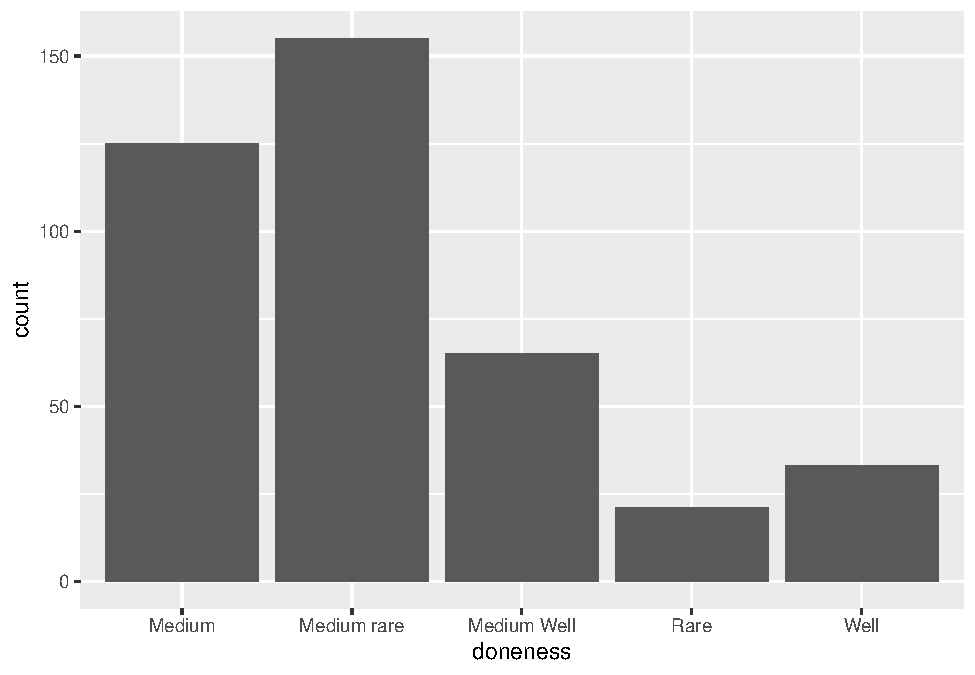
\includegraphics{how_americans_like_their_steak_files/figure-latex/barplot-1.pdf}

Calculate total risks taken by each individual.

\begin{Shaded}
\begin{Highlighting}[]
\NormalTok{non\_null\_risks[non\_null\_risks}\SpecialCharTok{==}\StringTok{\textquotesingle{}Yes\textquotesingle{}}\NormalTok{] }\OtherTok{\textless{}{-}} \DecValTok{1}
\NormalTok{non\_null\_risks[non\_null\_risks}\SpecialCharTok{==}\StringTok{\textquotesingle{}No\textquotesingle{}}\NormalTok{] }\OtherTok{\textless{}{-}} \DecValTok{0}

\NormalTok{change\_type }\OtherTok{\textless{}{-}} \FunctionTok{c}\NormalTok{(}\StringTok{\textquotesingle{}smoker\textquotesingle{}}\NormalTok{, }\StringTok{\textquotesingle{}alcohol\textquotesingle{}}\NormalTok{, }\StringTok{\textquotesingle{}gamble\textquotesingle{}}\NormalTok{, }\StringTok{\textquotesingle{}skydiving\textquotesingle{}}\NormalTok{, }\StringTok{\textquotesingle{}speeding\textquotesingle{}}\NormalTok{, }\StringTok{\textquotesingle{}cheated\textquotesingle{}}\NormalTok{)}

\NormalTok{non\_null\_risks }\OtherTok{\textless{}{-}}\NormalTok{ non\_null\_risks }\SpecialCharTok{\%\textgreater{}\%} 
  \FunctionTok{mutate\_at}\NormalTok{(change\_type, as.integer)}

\NormalTok{non\_null\_risks}\SpecialCharTok{$}\NormalTok{doneness }\OtherTok{\textless{}{-}} \FunctionTok{factor}\NormalTok{(non\_null\_risks}\SpecialCharTok{$}\NormalTok{doneness, }\AttributeTok{levels =} \FunctionTok{c}\NormalTok{(}\StringTok{\textquotesingle{}Rare\textquotesingle{}}\NormalTok{, }\StringTok{\textquotesingle{}Medium rare\textquotesingle{}}\NormalTok{, }\StringTok{\textquotesingle{}Medium\textquotesingle{}}\NormalTok{, }\StringTok{\textquotesingle{}Medium Well\textquotesingle{}}\NormalTok{, }\StringTok{\textquotesingle{}Well\textquotesingle{}}\NormalTok{))}

\NormalTok{non\_null\_risks }\OtherTok{\textless{}{-}}\NormalTok{ non\_null\_risks }\SpecialCharTok{\%\textgreater{}\%} 
  \FunctionTok{mutate}\NormalTok{(}\AttributeTok{total\_risks =}\NormalTok{ smoker }\SpecialCharTok{+}\NormalTok{ alcohol }\SpecialCharTok{+}\NormalTok{ gamble }\SpecialCharTok{+}\NormalTok{ skydiving }\SpecialCharTok{+}\NormalTok{ speeding }\SpecialCharTok{+}\NormalTok{ cheated)}
\end{Highlighting}
\end{Shaded}

Using a crosstab view, we can determine how people like their steak
within each region

\begin{Shaded}
\begin{Highlighting}[]
\NormalTok{knitr}\SpecialCharTok{::}\FunctionTok{kable}\NormalTok{(}\FunctionTok{crosstab}\NormalTok{(non\_null\_risks, }\AttributeTok{x =}\NormalTok{ us\_region, }\AttributeTok{y =}\NormalTok{ doneness, }\AttributeTok{weight =}\NormalTok{ total\_risks))}
\end{Highlighting}
\end{Shaded}

\begin{longtable}[]{@{}
  >{\raggedright\arraybackslash}p{(\columnwidth - 12\tabcolsep) * \real{0.2500}}
  >{\raggedleft\arraybackslash}p{(\columnwidth - 12\tabcolsep) * \real{0.1316}}
  >{\raggedleft\arraybackslash}p{(\columnwidth - 12\tabcolsep) * \real{0.1579}}
  >{\raggedleft\arraybackslash}p{(\columnwidth - 12\tabcolsep) * \real{0.1184}}
  >{\raggedleft\arraybackslash}p{(\columnwidth - 12\tabcolsep) * \real{0.1579}}
  >{\raggedleft\arraybackslash}p{(\columnwidth - 12\tabcolsep) * \real{0.1316}}
  >{\raggedleft\arraybackslash}p{(\columnwidth - 12\tabcolsep) * \real{0.0526}}@{}}
\toprule()
\begin{minipage}[b]{\linewidth}\raggedright
us\_region
\end{minipage} & \begin{minipage}[b]{\linewidth}\raggedleft
Rare
\end{minipage} & \begin{minipage}[b]{\linewidth}\raggedleft
Medium rare
\end{minipage} & \begin{minipage}[b]{\linewidth}\raggedleft
Medium
\end{minipage} & \begin{minipage}[b]{\linewidth}\raggedleft
Medium Well
\end{minipage} & \begin{minipage}[b]{\linewidth}\raggedleft
Well
\end{minipage} & \begin{minipage}[b]{\linewidth}\raggedleft
n
\end{minipage} \\
\midrule()
\endhead
East North Central & 0.000000 & 40.36145 & 33.73494 & 15.662651 &
10.240964 & 166 \\
East South Central & 0.000000 & 54.34783 & 23.91304 & 6.521739 &
15.217391 & 46 \\
Middle Atlantic & 11.510791 & 20.14388 & 36.69065 & 22.302158 & 9.352518
& 139 \\
Mountain & 0.000000 & 28.20513 & 39.74359 & 17.948718 & 14.102564 &
78 \\
New England & 5.333333 & 44.00000 & 34.66667 & 12.000000 & 4.000000 &
75 \\
Pacific & 8.510638 & 34.57447 & 38.82979 & 10.106383 & 7.978723 & 188 \\
South Atlantic & 6.666667 & 38.46154 & 26.66667 & 23.076923 & 5.128205 &
195 \\
West North Central & 11.578947 & 46.31579 & 29.47368 & 12.631579 &
0.000000 & 95 \\
West South Central & 0.000000 & 51.66667 & 26.66667 & 13.333333 &
8.333333 & 60 \\
\bottomrule()
\end{longtable}

\begin{Shaded}
\begin{Highlighting}[]
\NormalTok{grouped }\OtherTok{\textless{}{-}} \FunctionTok{crosstab}\NormalTok{(non\_null\_risks, }\AttributeTok{x =}\NormalTok{ us\_region, }\AttributeTok{y =}\NormalTok{ doneness, }\AttributeTok{weight =}\NormalTok{ total\_risks, }\AttributeTok{format =} \StringTok{\textquotesingle{}long\textquotesingle{}}\NormalTok{)}

\NormalTok{grouped }\SpecialCharTok{\%\textgreater{}\%} 
  \FunctionTok{ggplot}\NormalTok{(}\FunctionTok{aes}\NormalTok{(}\AttributeTok{x =}\NormalTok{ pct, }\AttributeTok{y =}\NormalTok{ us\_region, }\AttributeTok{fill =}\NormalTok{ doneness)) }\SpecialCharTok{+}
  \FunctionTok{geom\_bar}\NormalTok{(}\AttributeTok{stat =} \StringTok{\textquotesingle{}identity\textquotesingle{}}\NormalTok{, }\AttributeTok{position =} \FunctionTok{position\_fill}\NormalTok{(}\AttributeTok{reverse =} \ConstantTok{TRUE}\NormalTok{)) }\SpecialCharTok{+}
  \FunctionTok{xlab}\NormalTok{(}\StringTok{"Total Region \%"}\NormalTok{) }\SpecialCharTok{+}
  \FunctionTok{ylab}\NormalTok{(}\FunctionTok{element\_blank}\NormalTok{()) }\SpecialCharTok{+}
  \FunctionTok{geom\_text}\NormalTok{(}\FunctionTok{aes}\NormalTok{(}\AttributeTok{label =} \FunctionTok{paste0}\NormalTok{(}\FunctionTok{round}\NormalTok{(pct, }\DecValTok{0}\NormalTok{), }\StringTok{\textquotesingle{}\%\textquotesingle{}}\NormalTok{)), }\AttributeTok{position =} \FunctionTok{position\_fill}\NormalTok{(}\AttributeTok{reverse =} \ConstantTok{TRUE}\NormalTok{, }\AttributeTok{vjust =} \FloatTok{0.5}\NormalTok{), }\AttributeTok{size =} \FloatTok{2.5}\NormalTok{, }\AttributeTok{color =} \StringTok{\textquotesingle{}black\textquotesingle{}}\NormalTok{, }\AttributeTok{fontface =} \StringTok{\textquotesingle{}bold\textquotesingle{}}\NormalTok{) }\SpecialCharTok{+}
  \FunctionTok{scale\_x\_continuous}\NormalTok{(}\AttributeTok{labels =}\NormalTok{ scales}\SpecialCharTok{::}\NormalTok{percent) }\SpecialCharTok{+}
 \FunctionTok{theme}\NormalTok{(}\AttributeTok{legend.position =} \StringTok{"top"}\NormalTok{, }\AttributeTok{legend.title =} \FunctionTok{element\_blank}\NormalTok{()) }\SpecialCharTok{+}
  \FunctionTok{labs}\NormalTok{(}\AttributeTok{title =} \StringTok{\textquotesingle{}Steak Doneness by US Region\textquotesingle{}}\NormalTok{) }\SpecialCharTok{+}
  \FunctionTok{scale\_y\_discrete}\NormalTok{(}\AttributeTok{limits=}\NormalTok{rev) }\SpecialCharTok{+}
  \FunctionTok{scale\_fill\_brewer}\NormalTok{(}\AttributeTok{palette=}\StringTok{"RdBu"}\NormalTok{)}
\end{Highlighting}
\end{Shaded}

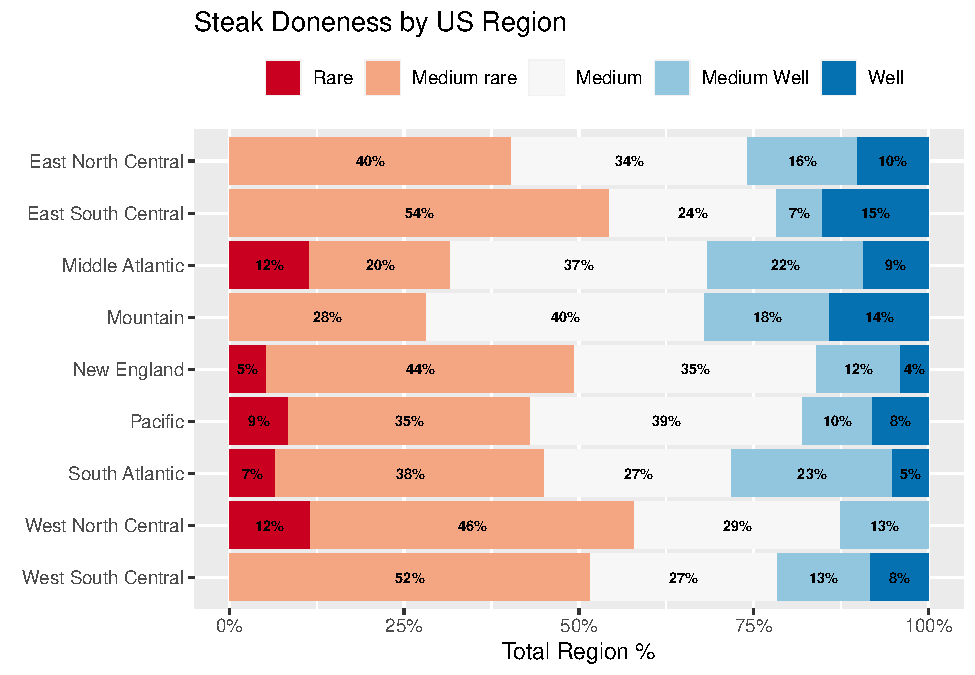
\includegraphics{how_americans_like_their_steak_files/figure-latex/grouped-us_region-doneness-1.pdf}

Surprisingly, not every region is represented by people who prefer their
steaks rare.

\hypertarget{recommendations}{%
\subsection{Recommendations}\label{recommendations}}

Given how the survey was taken, more information would be beneficial to
help determine riskiness. Each question only offered the options of
Yes/No, however, the degree of risk may vary based on frequency. A
person who drinks alcohol, may drink a few glasses per week, but another
person may drink several per day. The survey is also at risk of
self-selection bias and does not account for random sampling. Lastly,
are certain race/religions more prone to how they like to eat steak?

\end{document}
